\documentclass{scrreprt}
% coma version of report class:
% http://tex.stackexchange.com/questions/5948/subtitle-doesnt-work-in-article-document-class

\usepackage{fullpage}
\usepackage[utf8]{inputenc} % åäö
\usepackage{hyperref}
\usepackage{enumitem}
\usepackage[toc]{glossaries}
\usepackage{xcolor}
\usepackage{listings}
\usepackage{tikz}
\usetikzlibrary{calc, fit, shapes.geometric, arrows}
\pgfdeclarelayer{background}
\pgfdeclarelayer{foreground}
\pgfsetlayers{background,main,foreground}
\usepackage[T1]{fontenc}
\usepackage{ulem}
\usepackage{fancyvrb}
\usepackage{shorttoc}
\usepackage{epigraph}


\renewcommand*\contentsname{Contents (detailed)}


% Info about natbib:
% https://www.sharelatex.com/learn/Bibliography_management_with_natbib
% http://en.wikibooks.org/wiki/LaTeX/Bibliography_Management#Natbib
\usepackage[round]{natbib}
\bibliographystyle{plainnat}



\setkomafont{disposition}{\normalfont\bfseries}


% Remove date
\date{2014}

\hypersetup{
  colorlinks = true,
  linkcolor = black,
  citecolor = red
}

\title{ A language for expressing \\ descriptive markup languages }
\subtitle{A holistic response to constant \\ change in contemporary authorship.}
\author{ Christopher OKHRAVI \\ UPPSALA UNIVERSITY }


%
% Defining research questions
%
\newcommand\researchquestionformat[1]{\begin{quote}#1\end{quote}}
\newcommand\firstresearchquestion{\researchquestionformat{%
  \textbf{(RQ1) Research question 1} \\
  Can the verbosity of document annotation formats (e.g. \texttt{XML}) be decreased, by allowing authors themselves to design annotation formats?%
}}


\newcommand\secondresearchquestion{\researchquestionformat{%
  \textbf{(RQ2) Research question 2} \\
  Can an annotation language
  For an author to be able to design an annotation language, this author must design a domain-specific-language (DSL), a parser, a compiler and a transformation engine. Consequently we come to the point where we instead ask ourselves the following question:


  Can a \texttt{Domain Specific Language (DSL)} be defined, such that a semi-technical author can employ it to design a document annotation format?

  Requiring (A) the combined complexity of the DSL and the annotated document is less than that of a document annotated in a traditional markup language with fixed syntax (e.g. \texttt{XML}).

  Without (B) sacrificing any flexibility of the original markup language.
}}

\newcommand\thirdresearchquestion{\researchquestionformat{%
  \textbf{(RQ3) Research question 3} \\
  Can a process be defined, such that any document can be converted into \texttt{XML} format, using \texttt{Regular Expressions} as rules for document hierarchy?
}}

\newcommand\fourthresearchquestion{\researchquestionformat{%
  \textbf{(RQ4) Research question 4} \\
  Can a language be defined, such that it is a subset of \texttt{Regular Expressions}, where most control characters are replaced by assumptions? Where the intent of the subset is to express annotations of document hierarchy.
}}


\newcommand{\tab}{\hspace*{6pt}}
\newcommand{\tabb}{\tab\tab}



\newenvironment{example}
{ \hrulefill \vspace{12pt} \\ }
{ \\\\ \vspace{12pt} \hrulefill }


\lstset{
  language=XML,
  basicstyle=\color[rgb]{0.3,0.3,0.3}\ttfamily\scriptsize,
  backgroundcolor=\color[rgb]{0.98,0.98,0.98},
  showstringspaces=false,
  breaklines,
  breakatwhitespace,
}





%
%
%
% FANCY CHARACTERS
%
%
%
\newcommand*{\prim}{\ensuremath{\prime}} % Prime









%
%
% GLOSSARY
%
%

\newglossaryentry{document authoring}{
  name={Document Authoring},
  description={The act of writing literature.}
}
\newglossaryentry{EBNF}{
  name={EBNF},
  description={Extended Backus-Naur Form}
}
\makeglossaries







%
%
%
% TiKZ Figures
%
%
%
\tikzstyle{startstop} = [rectangle, rounded corners, minimum width=3cm, minimum height=1cm,text centered, draw=black, fill=red!30]
\tikzstyle{io}       = [trapezium, trapezium left angle=75, trapezium right angle=105, minimum width=2cm, minimum height=1cm, text centered, draw=black, fill=blue!30]
\tikzstyle{process}  = [rectangle, minimum width=2cm, minimum height=2cm, text centered, draw=black, fill=orange!30]
\tikzstyle{decision} = [diamond,   minimum width=2cm, minimum height=2cm, text centered, draw=black, fill=green!30]
\tikzstyle{arrow}    = [thick,->,>=stealth]












\begin{document}

\maketitle
\shorttoc{Contents}{1} % Only sections
\tableofcontents
\pagebreak





% % % % % % % % % % % % % % % % % % % % % % 
%
%
%
%    The linguistic note
%
%
%
% % % % % % % % % % % % % % % % % % % % % %
\chapter*{A linguistic note}
A linguistic note in the spirit of Scribe (1980).
 






% % % % % % % % % % % % % % % % % % % % % % 
%
%
%
%    Glossary
%
%
%
% % % % % % % % % % % % % % % % % % % % % %
\glsaddall
\printglossary






% % % % % % % % % % % % % % % % % % % % % % 
%
%
%
%     Introduction
%
%
%
% % % % % % % % % % % % % % % % % % % % % %

\chapter{Introduction}

Since the invention of the writing on the wall, mankind has struggled with an interesting problem of change. Be it change in medium or means (e.g. the process of production or the means of storage). Every generation bear the burden of passing the collective body of knowledge on to the next. Every generation that cause medium or means of the written word to significantly change --  face a somewhat trivial dilemma. To somehow transcend (transform) all existing written content to fit the new ways of today, or leave the currently collected body of human knowledge to slowly perish with time.

The writing in stone cannot possibly accommodate all of the existing human knowledge. This problem of space can for example be solved by moving content to books. Paper, however, is a biological material that deteriorate with time. Consequently we have a problem of degradation. Digital representations is utterly superior in that it can be almost instantly copied and duplicated. Consequently, a process of duplication may be sufficiently cheap so as to answer to the problem of material deterioration. Because of course, even hard drives, and flash disks deteriorate with time. In the digital world however, we face a problem of interoperability. New file formats are invented every day. Employing a naive process of constant duplication will leave our future selves in a position where some formats may be as costly to interpret as the ancient writing on the wall is to us today. As the native speakers of a language die, so does the knowledge uniquely encoded in that language.

Instead, I argue that the one sensible approach is to employ a constant rewriting of the complete body of written human knowledge. To ensure that no authored work is lost in the translation of time.

But the big problem is of course that this is an utterly massive undertaking. So massive that it is obviously absurd to assume this process should be carried out by humans. But not yet so massive that it would be absurd to ask computers to carry it out. This thesis suggests taking a holistic approach to the current body of markup languages, identifying the common intersection, and suggesting a structured way in which some subset of languages any of these languages can be transformed into any of these other languages (TODO! THIS IS NOT CORRECT). With less human effort required than today. And with more preparation for potentially new languages of the future.

\paragraph{TODO}
- A brief history of writing from pens, to the printing press, to computers and word processors, to markup languages.
 




\section{Problem outline}
\label{sec:problems}
The problem area of this thesis is probably best be summarized by a quote raised in a paper by \cite*{krijnen} on a different approach to a problem similar to the problem raised in this thesis.

\begin{quote}
``The nice thing about standards is that there are so many to choose from.''\\
\textit{-- Andy Tanenbaum}
\end{quote}

Because we have so many different formats, for various good reasons, the need to convert between these formats, for various good reasons, is apparent. Let us begin with some examples. A reason for why we have different input formats may be that we as individuals appreciate different approaches and ways of thinking and thus syntaxes. Another might be that some formats simply cannot express concepts that another format can express. A reason for why we would like to convert between formats could be that of publishing. Given the multitude of devices and programs that can consume our documents it should be in our interest to supply appropriate formats for these devices and programs. 

\paragraph{An existing approach} to this ``n-to-n'' conversion problem, and perhaps the most obvious one is Pandoc\footnote{http://johnmacfarlane.net/pandoc/} -- dubbed ``a universal document converter''. The problem I see with Pandoc however is it's lacking facilities for customization of the conversion process. Assume for example that we are converting a document expressed in Markdown to HTML. None of the formats natively support the concept of a Table Of Contents (TOC). Wanting to do this, we would have to ``intercept'' the program after it has parsed the input, and use Haskell or Python to transform the JSON representation of the Abstract Syntax Tree (AST). This interception possibility is not a ``hack'' but built in to the Pandoc system and referred to as Scripting\footnote{http://johnmacfarlane.net/pandoc/scripting.html}.

Thus, the issues related to Pandoc are two-faceted. On one hand (P1) it may be difficult for semi-programmers to significantly modify the structure of a output document, but on the other -- even (P2) assuming programmers would collectively build an extensive library of transformation scripts for Pandoc, these ``packages'' operate on AST's that represent already complex formats. This facility and it's drawbacks is made clear in the research of \citet{krijnen}, who propose a solution for essentially the same problem as this thesis. The main difference between the approach of this thesis and that of \citet{krijnen} is that they operate on a ``lower level''. Seemingly \citet{krijnen} operate with intents of compilation efficiency through the use of lazy-evaluation, and criticize the Pandoc scripting system for requiring multiple (thus costly) runs over the AST. While the work of \citet{krijnen} is splendid, I unfortunately argue that formal grammars are too complex for such a tool to be used by laymen, or semi-programmers.

To put this thesis in relation to Pandoc's Scripting facilities, the argument goes along the lines of readability for the masses. I am not arguing that the current approach of Pandoc is absurd -- in fact, argue the approach of \citet{krijnen} is beautiful from a composition point of view, and I argue that the approach of Pandoc is effective in getting around to solve the problem without too much fuss. In this thesis, we will however look at an approach I argue is even more fuss-free than that of Pandoc Scripting. This is why we talk about a holistic approach to markup languages. Subjectively I would argue that both Pandoc and the work of \citet{krijnen} are \emph{reactive} instead of \emph{proactive}. In this thesis we look at the intents of markup languages from a more abstract point-of-view, revisit the actual intents and needs and not simply argue that the problem is the need to convert all formats to all formats. That undertaking, I argue, is too huge to provide significant value -- yet (TODO -- unclear).

\begin{quote}
``If I had asked people what they wanted, they would have said faster horses.''
\begin{flushright}
% TODO Make sure all quotes are formatted alike
\textit{-- Commonly attributed to Henry Ford}
\end{flushright}
\end{quote}


\paragraph{Another existing approach} is to instead of regarding this as an ``n-to-n'', regarding it as a ``1-to-n'' problem. Expressing our documents in a single format but converting into any imaginable format. This approach has been utterly popularized and democratized through the family of languages under XML.

An author can express her document in an arbitrary XML-format (perhaps imagined ``on the fly''), and then use a combination of XSLT and XPath to convert this document into any other imaginable format. Some problems with this approach is (1) the verbosity of the XML languages\footnote{http://www.ibm.com/developerworks/xml/library/x-sbxml/index.html} \footnote{http://blog.codinghorror.com/xml-the-angle-bracket-tax/} \footnote{http://blog.codinghorror.com/revisiting-the-xml-angle-bracket-tax/}, and (2) the fact that because of the lack of any kind of centralization or standardization of format or process, reuse of common transformations become difficult. The composition problem becomes apparent again. Wouldn't you rather use an XML to PDF transformer that the community had curated rather than rewriting one from scratch? Rhetorical question. The problem is again that since XML allows for an infinite number of syntaxes it is non-trivial to encompass all these syntaxes in the transformer.

\paragraph{Of course there are XML subsets like DocBook} that are more commonly accepted than others. Thus, community curated packages exist that can convert between the commonly used format and some other common presentational format e.g. PDF\footnote{http://docbook.sourceforge.net/}. This makes the XML situation look very much like the Pandoc situation (TODO -- not entirely) but instead of considering completely different syntaxes as input, one considers the XML-based languages. The main problem with this approach is that the input format is fixed. If (e.g.) the Docbook format is not sufficiently rich to express some concept that the author want to express then the community curated converter will be of limited use. Thus, that is a problem with diverging input. In the other end, we can look at diverging output. If working with standards, it is reasonable to assume that there is a standardized (or set of standardized options) for output. What if the author wishes to diverge from the standard output style? How much is flexible and configurable?

\paragraph{Instead} this thesis suggest to employ a view of \texttt{M-to-N}, where \(number-of-languages-in(M) < number-of-languages-in(N)\). Where \(M\) is the body of  languages imagined by authors, declaratively expressed at the highest level of abstraction possible for the given domain, and \(N\) is the set of all potential languages the author might want to convert the input into. Where all languages in \(M\) must lie in the intersection of all the languages in \(N\). In other words \texttt{\(M \subset (N_1 \cup N_n) \)}. 

In this thesis I will argue that there is a difference between converting a document when the language is within M, from M to N, or within N. I will also argue that employing this division will spawn much more pragmatic solutions than many-to-many-document conversions.

\paragraph{The aim} of this thesis, is to suggest a software eco-system\footnote{TODO -- need to define term?} in which a document author can ``write once, [and] publish everywhere''. But of course, that is an oversimplification. More specifically this thesis suggest a way in which we could write our (1) actual document contents once, (2) the transformation process in which we create, what \citet{reid} refers to as, ``derived text'' once, and finally (3) the mapping onto an output format once (per format of course). Note that the two second parts are generalized, and could be published as packages and reused. Also this is an oversimplification as we're going to need some ``glue'' as well. What also is not obvious in the above explanation is that this thesis suggest an approach that can be likened by a pipeline of templates (similar to a UNIX pipe\footnote{http://en.wikipedia.org/wiki/Pipeline\_(Unix)}) and through this achieve a high level of composability. Instead of a one-pass-transform, transformations are split into composable chunks at different levels of abstraction. But all this will be discussed further on in the thesis.






% TODO: Use or remove?
%\paragraph{Existing solutions}
%\begin{itemize}
%\item No proper pipeline for reusing common things, such as the creation of a table of contents.
%\item Could be solved using e.g XSLT but too verbose. No standard way of sharing libs.
%\item Pandoc is too difficult to configure. Syntax. Haskell/Python. Lacks an approach to share libs. 
%\end{itemize}



\section{Requirements}
Given the holistic problem outlined in Section \ref{sec:problems}, we will discuss a holistic response, in form of an eco-system of tools. In order to guide the development of the tool-chain, the following requirements have been extracted from the problems outlined in Section \ref{sec:problems}.

\paragraph{Any output format but reasonable input format}
As an author I must be able to author my document once, in a ``reasonable'' format. However, as an author, I must be able to publish to multiple platforms -- without \emph{any} rewriting. However, minor configuration must be allowed in order to ensure flexibility in output.

\paragraph{Composable} or code reuse through package friendliness. Code reuse must be a top priority. Not merely within an author's workflow of a single document, but also between authors and documents. Consequently, as much as possible must be able to be distributed as packages. \footnote{TODO -- call it composability or modularity?}

\paragraph{Extendable} refers to the idea that it must be natural to introduce new packages that intercept the process at any point in time. This requirement encompass the idea that authors must be offered control over the production of the final output.

\paragraph{Declarative}
All code that an eco-system user would touch must be declarative. Also packages must be expressed declaratively. This encompass the idea of using template transformations rather than imperative processing.




\section{Thesis outline}
TODO.



























% % % % % % % % % % % % % % % % % % % % % % 
%
%
%
%     Theory
%
%
%
% % % % % % % % % % % % % % % % % % % % % %


\chapter{Background}
Lorem ipsum. TODO.




\section{A brief history of Markup}

\begin{tabular}{ l | l | l | l }
  \textbf{Year} &
  \textbf{Language} &
  \textbf{Semantic-free} &
  \textbf{Mixed-content}
  \\ \hline

  1967 &
  \href{http://en.wikipedia.org/wiki/RUNOFF}{RUNOFF, ROFF}

  \\ \hline
  1969 &
  \href{http://en.wikipedia.org/wiki/IBM_Generalized_Markup_Language}{GML}

  \\ \hline
  1973 &
  \href{http://en.wikipedia.org/wiki/Nroff}{NROFF}

  \\ \hline
  1978 &
  TeX

  \\ \hline
  1980 &
  \href{http://www.dtic.mil/docs/citations/ADA125287}{Scribe}

  \\ \hline
  1986 &
  \href{http://en.wikipedia.org/wiki/SGML}{SGML}

  \\ \hline
  1979 &
  \href{http://www.troff.org/history.html}{TROFF}

  \\ \hline
  1990 &
  \href{http://en.wikipedia.org/wiki/Groff_(software)}{GROFF}

  \\ \hline
  1991 &
  \href{http://alistapart.com/article/a-brief-history-of-markup}{HTML}

  \\ \hline
  1992 &
  \href{http://en.wikipedia.org/wiki/Setext}{Setext}


  \\ \hline
  2000
  & \href{http://public.ccsds.org/publications/archive/641x0b2.pdf}{Parameter Value Language}
  & ??

  \\ \hline
  2002 &
  \href{http://en.wikipedia.org/wiki/Asciidoc}{AsciiDoc}

  \\ \hline
  2003 &
  \href{http://en.wikipedia.org/wiki/Org-mode}{OrgMode}

  \\ \hline
  2004 &
  \href{http://en.wikipedia.org/wiki/Markdown}{Markdown}+


  \\ \hline
  &
  \href{http://en.wikipedia.org/wiki/Textile_(markup_language)}{Textile 2} (TODO: 1?)
\end{tabular}


- What does it mean to annotate? What are common document annotation formats?

- Examples of markup languages and showcase of some syntax examples.

- A brief overview of markup languages and how they can be used for (1) Document authoring, and (2) Data transport.

- The relevance of markup for fiction and non-fiction.



\section{Mixed content}
When discussing markup languages -- I often find the need to make a distinction between intentions of (1) \emph{data modeling} and (2) \emph{document authoring}. One could of course argue that any imaginable document (in the document authoring sense) could be encoded in a particular data structure. That is however not the argument I am opposing here. I argue that some languages are more suited for intermingling non-marked up text with marked up text.

% TODO: Use and refer to the terms used by H. Schöning (2001) -- Tamino a DBMS for XML.

The first official W3C working draft of XML (1996)\footnote{http:\/\/www.w3.org/TR/1998/REC-xml-19980210\#sec-mixed-content} already contained the idea of what was referred to as ``mixed content''. Simplified, the idea was that an element may either contain a string of text, or another element, or any combination of the two. In (1998) W3C published a recommended specification of XML 1.0, where the concept of mixed content was expressed as a grammar in Extended Backus-Naur Form (subsequently referred to as EBNF) as follows\footnote{Part of the production for the non-terminal ``content'' has been omitted in favor of readability.}.

\begin{lstlisting}
element ::= EmptyElemTag | STag content ETag 
content ::= (element | CharData)*
\end{lstlisting}

In essence -- any non-terminal \texttt{element} can either produce an \texttt{EmptyElemTag} (i.e. self-closing tag), or the set of a \texttt{STag} (i.e. opening tag) followed by \texttt{content}, followed by an \texttt{ETag} (i.e. closing tag). The non-terminals \texttt{start} (e.g. \texttt{<foo>}) and \texttt{end} (e.g. \texttt{</foo>}) will terminate without any risk of indirect recursion back to the non-terminal \texttt{element}. The non-terminal \texttt{content} is the one interesting to this example.

In the XML 1.0 (1998) specification the following is true\footnote{This is of course merely a partial extraction of the syntax used in the specification.} for the EBNF syntax. The character ``pipe'' (|) represent an \texttt{XOR} choice such that \texttt{A | B} match ``A or B but not both''. The character ``star'' (*) is used as a ``Kleene Star'' such that \texttt{A*} matches ``zero or more occurrences of A''. Parentheses is used to group expressions such that the two mentioned operators can be used on an expression group.

This essentially mean that the non-terminal \texttt{content} can produce either a new \texttt{element} (causing indirect recursion) or \texttt{CharData} (i.e. a string), any number of times. Subsequently allowing for any combination of any length of the two.



\subsection{Exploring an example of mixed content}
I argue, that Mixed content is a fundamental, and necessary, property of markup languages. The following example is partially intended to help enforce this. Assume we have a formatted paragraph of text\footnote{In this example we will disregard whitespace between tokens and assume that whitespace between words in a string remains, but whitespace between strings is omitted and left implicit.}, as outlined in Figure \ref{fig:mixed-content-paragraph}.


\begin{figure}[h]
\centering
\fbox{
The color \underline{is \textbf{now}} \sout{red}.
}
\caption{An example paragraph with formatting.}
\label{fig:mixed-content-paragraph}
\end{figure}


Assume that we want to mark up some aspects of the formatting. The important\footnote{...and admittedly fabricated...} characteristics are that the paragraph, from a markup perspective, can be argued to consist of four unique ``token types''. More precisely (1) plain-text, (2) underline, (3) bold and underline, and finally (4) strike-through.


More importantly, the fact that two words are underlined, whereas one of those words are both underlined and drawn in bold. When working with markup, this situation is usually expressed through inheritance. This is visualized in Figure \ref{fig:mixed-content-tree}. Without inheritance, the number of tokens needed in our lexer would have to be the number of permutations of \texttt{n} (i.e. \texttt{n!}) where \texttt{n} is the number of unique tokens.




Assume we had a lexical analyzer (onwards referred to as ``lexer'') that could read this visual markup. Obviously this is a purely hypothetical lexer as it will be able to identify beginnings and endings of visual markup. Consider for example the human vision and mind. Or an OCR (Optical Character Recognition) engine. A sensible tokenization from this lexer's point of view might go along the following lines (where tokens prepended with \texttt{S-} represents ``starting of'' and \texttt{E-} ``ending of''),




\begin{lstlisting}
  TXT S-UNDERLINE TXT S-BOLD TXT E-BOLD S-STRIKETHROUGH TXT E-STRIKETHROUGH TXT
\end{lstlisting}



Figure \ref{fig:mixed-content-tree} visualizes a reasonable parse-tree in pre-order. In which ending of a particular property is simply denoted by not being a child of that parent. In the figure, the nesting of properties, becomes obvious.
  



\begin{figure}[h]
  \centering
  \begin{tikzpicture}[
    tlabel/.style={pos=1,right=2pt,font=\footnotesize\color{red!70!black}},
    sibling distance=4cm,
  ]
  \node {<root>}
  child {node {"The color"}}
  child {node {<underline>}
    child {node {"is"}}
    child {node {<bold>}
      child {node {"now"}}
    }
  }
  child {
    node {<strikethrough>}{
      child {node {"red"}}
    }
  }
  child {node {"."}}
  ;
  \end{tikzpicture}

  \caption{The example paragraph from \ref{fig:mixed-content-paragraph} represented as a pre-order tree.}
  \label{fig:mixed-content-tree}
\end{figure}



Now that we have established an example input, a model tokenization and a model parse-tree, let us attempt to express this in two different languages.



\subsubsection{Suitable formats for Mixed Content}
Figure \ref{fig:mixed-content-paragraph} in XML.


\begin{figure}[h]
\begin{lstlisting}
The color <underline>is <bold>now</bold> <strikethrough>red</strikethrough>.
\end{lstlisting}
\caption{Expressing Figure \ref{fig:mixed-content-paragraph} in XML.}
\label{fig:mixed-content-xml}
\end{figure}



\subsubsection{Unsuitable formats for Mixed Content}
Mixed content becomes utterly difficult to express in languages that lack a canonical way of expressing it. Attempting to express Figure \ref{fig:mixed-content-paragraph} in JSON, one quickly realizes there are multiple ways and that it is not obvious which was is the one to prefer. No approach I have found\footnote{I have merely conducted non-scientific experiments.} is trivial to parse without telling the parser a particular piece of information.

\begin{figure}[h]
\begin{lstlisting}
{
  "root": [
    "The color ",
    { "emph": ["is", { "keyword": "red" }], },
    "now."
  ]
};
\end{lstlisting}
\caption{Attempting to express Figure \ref{fig:mixed-content-paragraph} in JSON.}
\label{fig:mixed-content-json}
\end{figure}


Consider Figure \ref{fig:mixed-content-json}. At first glance it seems like a perfectly reasonable representation of the discussed paragraph. Using Arrays to sequence, and single-key objects to name elements. However, the limitations become painfully apparent if we ask ourselves the question -- what does an object with two keys represent?

One might argue that the counter example is breaking the rules. We did say ``single-key objects'' and not ``n-key objects''. This is a syntactical requirement that can easily be encoded into the parser (or probably even the lexer). This is however to misunderstand the point. The point is that the JSON specification does not actually enforce this behavior today. Meaning, there is (to my knowledge\footnote{TODO: Do I need a reference or something?}) no way of representing mixed content with labeled elements using JSON, without introducing a requirement which isn't already encoded in the lexer/parser. Meaning, all valid JSON strings, cannot (applying a certain strategy, such as e.g. Figure \ref{fig:mixed-content-json}) be considered valid strings of mixed content. Ergo, JSON is an unsuitable format for mixed content.

Within this thesis, it is this line of reasoning that is referred to when discussing whether a particular format is suitable for representing mixed content or not.




\subsection{Enforcing the importance of mixed content}

Mignet et al. (2003) analyzed different aspects of what they referred to as ``The XML web'' (i.e. "the subset of the Web made of XML documents only"). During this study it was found that 72\% of all documents utilize mixed content. Almost three out of four documents use mixed content. Mignet et al. (2003) conclude that they invalidate the folklore which underestimate the importance of mixed content in XML. Given that XML (in contrast to HTML -- the de facto language of the web) is commonly used a data transportation format, one can reasonably assume that the number of HTML documents making use of mixed content is even higher.



Further, anyone who has ever authored a free-text-oriented document in a markup language of the XML-family (counting improper HTML subsets such as HTML5) I expect have some appreciation of how absurd document creation would be without mixed content.





\subsection{Old stuff TODO}
Markup is not just data transportation. An explanation as to why object notation is a subset of annotations. Meaning that formats like \texttt{JSON} are too data-centric and can consequently not, in any sensible manner, be used for manual document authoring. \texttt{XML} for example can be used for data transport, but in this thesis we'll focus on its markup properties. Consequently also ignore formats like \texttt{JSON}, \texttt{YAML} etc.

Maybe we can even use parse-tree's to symbolize the problem. To show that it is not possible to unambiguously represent mixed content. One needs to perform computation on the parse tree to derive the data.






\section{A Taxonomy of Markup Languages}
\label{sec:taxonomy}
In \citeyearpar{coombs} \citeauthor*{coombs} published an article dubbed \textit{Markup Systems and the Future of Scholarly Text Processing}. While the intent of the article, presumably, was to speculate on the future markup -- it also provided a solid taxonomy of markup languages. This thesis utilize the categorizations of ``types of markup'' identified by \citet{coombs}, under the term ``markup theory''. \citet{coombs} divide markup types into five categories.The categories are (1) Punctuational, (2) Presentational, (3) Procedural, (4) Descriptive, and (5) Abstract. We will now take a closer look at each of these.

Intermingled in these explanations are also opinions from \citeauthor{bray} (co-founder of the Open Text Corporation, and co-author of the first XML 1.0 draft specification) as expressed in a blog post \citeyearpar{bray} exploring the categorizations of \citet{coombs}. It is because of \citet{bray} I have decided to refer to the work of \citet{coombs} as a taxonomy.


\subsection{Punctuational}
Punctuational markup refer to the markup we pay little attention to in our everyday life. Spaces, commas, periods, words, sentences etc. As \citet{coombs} points out, punctuational markup has been studied by mankind for hundreds of years. The example \citet{coombs} use to underline that punctuational markup should, indeed, be considered markup and not merely a part of our writing system -- is the following. Consider the all the conflicting opinions on how punctuational markup should be used. You argue it ought to be a  semicolon, I argue it should be a colon. I argue space-delimited dash, you argue dash with no space. Consider the author contemplating whether a certain domain of sentences/words should be presented as \textbf{bold} or as \textit{italics}. This is the same kind of choice, as the mentioned choices between semicolon, colon and so forth. However, today, \textbf{bold} and \textit{italics} can clearly be considered markup, if you consider languages such as HTML.

Understand, that the term punctuational markup, according to \citet{coombs}, does not refer to the idea of encoding punctuation in some other language (i.e. ``\texttt{\&mdash;}'') but rather the actual punctuation itself (i.e. ``\texttt{--}''). In other words, the use of for example character entities in HTML5\footnote{http://dev.w3.org/html5/html-author/charref} is not to be considered punctuational markup.




\subsection{Presentational}
Assume we are talking about a document written on a very old, mechanical typewriter. Presentational markup, according to \citet{coombs} refer to the practice where the author of a document (e.g.) hit the space key multiple times to center text on the page. Or hitting enter multiple times to create paragraphs, or line-breaks.

Now, consider a physical paper document written with a ball pen by hand. With a little bit of effort the author can easily distinguish two parts of the text by applying the technique of writing in italics, or even in cursive. So the reader of the document would understand that author is attempting to communicate some semantic difference between the non-italic and the italic parts.

To understand presentational markup, consider the two above cases -- the typewriter document and the handwritten document. In both cases the presentational elements is embedded within the language of the document. The semantics intended by the author (e.g. a paragraph break) is achieved through presentational means.

\citet{bray} makes the concept of presentational markup, more clear by referring to older What You See Is What You Get (WYSIWYG) word processors. Since modern word processors work with (e.g.) descriptive markup ``under the hood'', this analogy generally no longer holds. But for the sake of the argument, imagine a really old version of e.g. Microsoft Word. But instead, consider word processors of the older model. By surrounding parts of a document with code specific to a particular word processor that particular word processor would know to (e.g.) display that piece of text centered, in bold, in italics or so forth.

One immediate problem with this, the quick reader probably have noticed, can be extracted from one particular sentence -- ``a specific word processor''. Presentational markup requires standardization of what codes to use to mark things such as bold, breaks, sizes and so forth. As you can probably imagine, with the creativity of programmers this quickly gets out of scale.

\subsubsection{Implicitness}
Another more subtle issue, not mentioned by neither \citet{coombs} nor \citet{bray}, is that of implicitness. As the presentational codes of WYSIWYG word processors are not actually visible to the user of the interface -- there exist a mental disconnect. Consider for example the concept of a paragraph break, and the concept of a hard line-break. Now, assume that, in a particular editor, a paragraph break has the same visual appearance as two consecutive hard line-breaks. Assume I type up a document, and hand it to you. How would you then possible know whether I have used paragraph breaks or hard line-breaks? Perhaps, this is the problem \citet{bray} is referring to, when arguing that What You See Is What You Get essentially is a false claim.



\subsection{Procedural}
The notion of Procedural markup is perhaps most easily communicated through making an analogy to procedural programming languages. Procedural markup refers to the idea of embedding instruction style code directly in the document. Much like as in procedural languages, code duplication, or painful repetition, \citet{bray} argue, can be reduced through elaborate macros or subroutines.

This is the first category that we have discussed, that actually show the user an abstraction of a particular concept rather than the actual concept. Assume an author is to write a particular sentence in a red font. If done through presentational markup, the user would actually see the sentence in red. If however done through procedural markup the user might something similar to Figure \ref{fig:procedural-markup-red-sentence}.


\begin{figure}[h]
\centering
\fbox{
\texttt{
  \textbackslash begin\{red\} This is a red sentence. \textbackslash end\{red\}
  }
}
\caption{A fictive example of procedural markup.}
\label{fig:procedural-markup-red-sentence}
\end{figure}


\begin{figure}[h]
\centering
\fbox{
\texttt{
  .sk 3 a;.in +10 -10;.ls 0;.cp 2 Multiple instructions.
  }
}
\caption{An example of procedural markup, as given by \citet{coombs}.}
\label{fig:procedural-markup-coombs}
\end{figure}



But depending on the syntax of the language, procedural markup might also turn out like a mess of symbols where the compiler instructions are hard to tell from the actual plain-text -- for the untrained professional of course. \citet{coombs} gives an example of procedural markup, as can be seen in \ref{fig:procedural-markup-coombs}, and suggest that the instructions should be interpreted as follows:

\begin{enumerate}
\item Skip three lines -- the equivalent of double-spacing twice.
\item Indent ten columns from the left and ten columns from the right.
\item Change to single-spacing.
\item Start a new page if fewer than two lines remain on the current page.
\end{enumerate}

We will discuss syntax in greater length further on. However, please consider the mental distance between syntax and the actual effect, for a minute. Consider how easy (or hard) it would be for a semi-technical author to remember and properly interpolate these commands into a document. I would argue that it is all but trivial.


\subsubsection{Mutation}
An interesting problem that reasonably may cause mental overhead for a document author working with procedural markup, is one of side-effects. Arguably, the notion of ``mutation'' or ``side-effects''\footnote{I use the terms ``mutation'' and ``side-effects'' interchangeably. TODO: Is that reasonable?} is a great source of power in programming, but also a great source of frustration. Programs that frequently mutate are generally tricky to debug\footnote{TODO Reference? Is it really true?}.

The same is true for procedural markup. With the syntax of Figure \ref{fig:procedural-markup-red-sentence} the text that differs from the ``default'' (i.e. the red text) is enclosed between two language constructs that mark its beginning and end. Admittedly, the behavior of the particular code snippet would be reasonably easy to predict, probably even for a semi-technical author. In the case of Figure \ref{fig:procedural-markup-coombs} however, the language construct is an instruction that mutate the state of the current document from that point and onwards. In a 200 page document with this syntax, it would suddenly be non-trivial to tell whether a particular instruction have cascaded down to a particular point or not.
%TODO: Should I rather use the term control statement

Consider the simple case where a number of words are marked up such that their font color will be red. A metaphor for the syntax of Figure \ref{fig:procedural-markup-red-sentence} would be equivalent to ``change to the red pen, and then change back to whatever pen you had before'', whereas the syntax of Figure \ref{fig:procedural-markup-coombs} merely would say ``change to the red pen''. Obviously this may cause confusion for a document author.




\subsection{Descriptive}
Unfortunately there seems to be no unanimous line between procedural and descriptive markup. \citet{coombs} argue that languages such as \TeX{} and \LaTeX{} are descriptive languages, whereas \citet{bray} argue they are procedural. If I am to speculate, I would assume this particular difference in opinion stems from the differences in state-of-the-art practice at the time in which these two publications were authored.

% In order to gain some understanding in why ambiguity might arise -- ask yourself the following question. If a language L, has a declarative syntax (meaning it cannot possibly be procedural), yet the declarative-style syntax clearly describes presentational... TODO: This is not a good example.

In the time of \citet{coombs}, languages like SGML were still fresh out of the oven (the ISO standard for SGML was published in 1986\footnote{http://www.iso.org/iso/catalogue\_detail.htm?csnumber=16387}). So the mere fact that the language provided a way of expressing parts of the document through description rather than through procedure, seemingly was enough for the language to be called descriptive. In other words, I speculate that at that time it was sensible to consider a markup language to be descriptive, so long as it showed significant descriptive capabilities. Regardless of whether it also provided ways of expressing procedural markup. In the case of \LaTeX{}, consider for example language constructs such as \texttt{\textbackslash vspace} (i.e. a command that inserts vertical space) -- clearly procedural.

Put this in contrast to the time of \citet{bray}, where languages like XML had succeeded SGML and provided almost purely descriptive facilities. In other words, I argue that markup languages at this point in time, could only be considered descriptive, if they \emph{only} allowed for descriptive (and never procedural) expressions.

Understand, that attributing this difference of opinion to the different contexts at those points in time, is of course completely speculative from my part. Reasonably so I would argue however.

Following in this thesis I will use a notion of descriptive markup, more similar to that of \citet{bray}. Following the definition both stated by \citet{coombs} as well as \citet{bray} -- that descriptive markup denotes what a given part of the document \emph{is} rather that what it \emph{does}. I.e. denoting what parts of the text belong to which class. However, realizing that the mistake I argue \citet{coombs} made, was allowing languages with both procedural and descriptive capabilities to be called descriptive. In this thesis a markup language exhibiting any kind of procedural element will be considered a procedural markup language, regardless of its descriptive capabilities.


\subsection{Referential}
Another category of markup described by \citet{coombs} is referential markup. The idea of referential markup essentially encompass the idea that we at some point (P1) in our document want to be able to include another part of a document or some string of characters (P2). Regardless of whether P1 and P2 are specified in different documents or even different machines.

Returning to the previously mentioned example with the character entity \texttt{\&mdash;}. If treated as referential markup, we might want every occurrence of that character entity (i.e. that piece of referential markup) to be replaced by the actual character ``\texttt{--}''.

\citet{coombs} argue that referential markup can exist in both procedural markup languages and descriptive. In the first it may take the form of user-defined variables. Whereas in the second, the case of character entity replacement outlined above is a prime example.


\subsection{Metamarkup}
Metamarkup is the term \citet{coombs} use to refer to markup languages that specify, extend, and/or constraint markup languages. While not explicitly mentioned by \cite{coombs} (as they were invented later\footnote{TODO is it true? refs?}), languages such as DTD (Document Type Definition), XML Schema, and RelaxNG are all metamarkup languages.

From a linguistic point of view, a metamarkup language can be seen as a metalanguage\footnote{http://en.wikipedia.org/wiki/Metalanguage} used to formally discuss an object language. Where in a concrete example the first could be RelaxNG and the second XML.




\section{A hierarchy of abstraction}
It is important to understand that \citet{coombs} employ the wording ``types of markup'' when discussing the categories explained in section \ref{sec:taxonomy}, whereas \citet{bray} discuss ``a taxonomy of markup''. While similarly sounding indeed, nuances emerge when considering the fact that \citet{bray} only discuss three of the total six categories outlined by \citet{coombs}. The three included in the, so called, taxonomy are (1) presentational, (2) procedural, and (3) descriptive.

If you would, again, allow me to speculate, then I would argue this stems from the way these three categories nicely describe three different levels of abstraction given an instance of a document. Or to look at it from the other end, consider the following. Punctuational markup can very well be expressed using presentational markup, as well as procedural, as well as descriptive. Referential markup can be expressed using the two latter, and the same goes for metamarkup.

In essence -- punctuational, referential and metamarkup are essentially concepts that \emph{can be expressed}. Whereas presentational, procedural and descriptive markup are \emph{ways to express} these concepts (amongst others).

Allow me to stress again, that this is my subjective interpretation of the situation. But consider it for a moment and I assume you also will find it reasonable. Consider for example how machine code can be abstracted into procedural code, and how procedural code can be abstracted into declarative. Then consider how this analogy conveniently align with the types of markup.


\begin{figure}[h]
\centering

  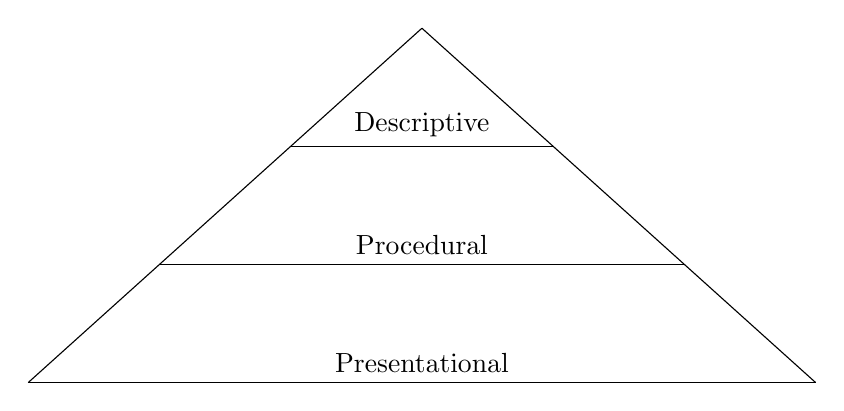
\begin{tikzpicture}
  \coordinate (Descriptive) at (-5,0) {};
  \coordinate (Procedural) at ( 5,0) {};
  \coordinate (Presentational) at ( 0,4.5) {};
  \draw (Descriptive) -- (Presentational);
  \draw (Procedural) -- (Presentational);
  \foreach \y/\Descriptive in {0/Presentational, 1/Procedural, 2/Descriptive} {
      \draw ($(Descriptive)!\y/3!(Presentational)$) -- ($(Procedural)!\y/3!(Presentational)$) node[midway,above] {\Descriptive};
  }
  \end{tikzpicture}

\caption{A hierarchy of markup language abstraction.}
\label{fig:markup-types-hierarchy}
\end{figure}



Consequently I argue that these three ``categories'' of the taxonomy can be viewed as paradigms of markup abstraction. Much like we have invented facilities to abstract away machine level instructions, we have invented facilities to abstract low level instructions for document content transformation. This hierarchy is visualized in Figure \ref{fig:markup-types-hierarchy}.  


% We are talking about _instances_ of documents, which is why we are not regarding abstract markup languages.








\section{Workflows}
In the spirit of \citet{reid} -- author of the paper that introduced Scribe, one of the earlier document preparation systems that argued for the ``separation of form from content'' -- we will now take a look at some popular workflows of document authoring. Further I will suggest an ideal alternative, targeting some of the apparent deficiencies with the current ones.

The process that we are going to analyze is that of file format transformation. The idea of transforming a file expressed in some format F into some other format F\prim.

Given the creativity of humans, I would argue that, the number of workflows used in the real world today is likely equivalent or higher than the number of people employing a workflow. Thus, in order to be able to discuss workflows, we need some way to generalize the concepts that are present in all. Thus, Figure \ref{fig:workflows-framework} suggests a micro-framework I will use as a basis for this discussion. Given it's high level of abstraction I strongly believe you will agree on it being representative for the whole set of potential workflows.

Think about it, to perform the process described as transforming from \texttt{F} to \texttt{F\prim}, we obviously need to be able to distinguish the two formats from each other. In Figure \ref{fig:workflows-framework} \texttt{F} is referred to as ``Input file'' and \texttt{F\prim} as ``Output file''. Further, we know that \texttt{F}, representing a static file format, never will transform itself into a the other static file format \texttt{F\prim}. Consequently we need some process in-between, in Figure \ref{fig:workflows-framework} we refer to this process as the ``Transformation program''. The figure then, I argue is general enough to encompass every reasonable and imaginable transformation workflow.

You might argue that some workflows actually encompass multiple steps of transformation, and I would of course agree. If you however consider how Figure \ref{fig:workflows-framework} actually depict a function, then it becomes obvious how we could use the output of one function as input to another function. Consequently, the model implies that you may apply it any number of times.


\subsection{Generality of the transformation program}
Unfortunately, the model depicted in Figure \ref{fig:workflows-framework} model is not sufficiently exact for our purposes. With it, we will not be able to illustrate the kind of distinctions we want to depict. Assume that we instead of having the two formats \texttt{F} and \texttt{F\prim}, have the four formats F. 




\begin{figure}[h]
  \centering

  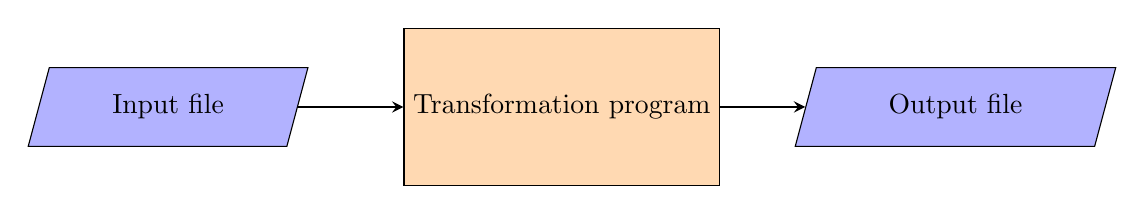
\begin{tikzpicture}[node distance=2.5cm]
    \node (input)  [io] {Input file};
    \node (engine) [process, right of=input, xshift=2.5cm] {Transformation program};
    \node (output) [io,      right of=engine, xshift=2.5cm] {Output file};

    % arrows
    \draw [arrow] (input)  -- (engine);
    \draw [arrow] (engine) -- (output);

    \begin{pgfonlayer}{background}
      % \node [draw, fill=cyan!25, rectangle, rounded corners, fit={(input) (engine) (output)}] { Foobar };
    \end{pgfonlayer}

  \end{tikzpicture}

  \caption{A naive interpretation of the problem of file transformation.}
  \label{fig:workflows-framework}
\end{figure}




\begin{figure}[h]
  \centering

  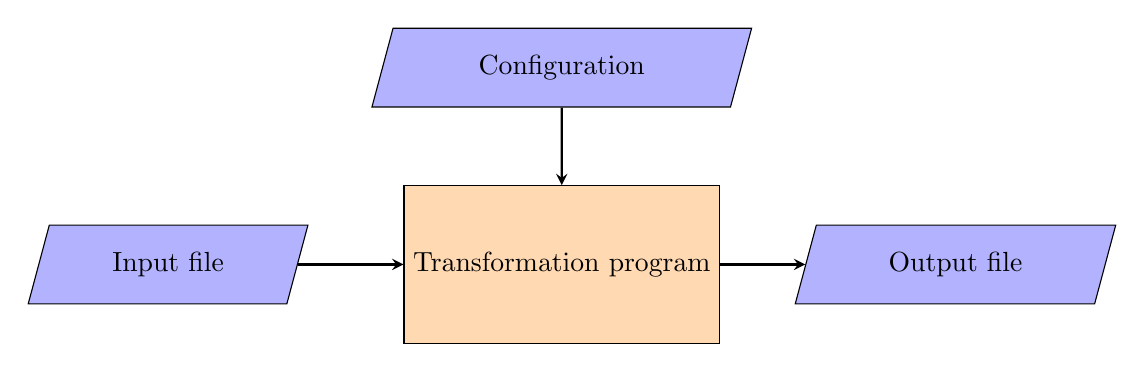
\begin{tikzpicture}[node distance=2.5cm]
    \node (input)  [io] {Input file};
    \node (engine) [process, right of=input, xshift=2.5cm] {Transformation program};
    \node (output) [io,      right of=engine, xshift=2.5cm] {Output file};
    \node (conf)   [io,      above of=engine]{Configuration};

    % arrows
    \draw [arrow] (input)  -- (engine);
    \draw [arrow] (engine) -- (output);
    \draw [arrow] (conf)   -- (engine);
  \end{tikzpicture}

  \caption{A micro-framework for discussing generality in document transformation. }
  \label{fig:workflows-framework}
\end{figure}











\section{Situational analysis}
Why are so many documents still procedural?
Model information flows of contemporary publishing. Figures describing the current state in contrast to the thesis's subjective idea of the ideal state. Refer to Reid (1980).

\subsection{Presentational}
i.e. Microsoft Word etc.
[FIG. ]
Explicit outline of the problems so that we can attack them in the hypothetical ideal.

\subsection{Procedural}
i.e. \LaTeX etc.
[FIG. ]
Explicit outline of the problems so that we can attack them in the hypothetical ideal.

\subsection{Descriptive}
i.e. DocBook, EPUB, Markdown etc.
[FIG. ]
Explicit outline of the problems so that we can attack them in the hypothetical ideal.

\subsection{A hypothetical ideal addressing the problems}
[FIG.]

\subsubsection{Composition \& Abstraction}
The minimal denominator.






















\chapter{Literature review}
Lorem ipsum.






\chapter{Empirics}
Lorem ipsum.


\section{SimEx -- A control structure-light subset of regex}
...


\section{Flexup -- A DSL for expressing markup-oriented CFG's}
...

\subsection{The annotated file (\texttt{.fup})}
...

\subsection{The annotation definitions file (\texttt{.fupd})}
...

\subsection{The binary}
...





\chapter{Analysis}
Lorem ipsum.





\chapter{Conclusion}
Lorem ipsum.





\chapter{Discussion}
Lorem ipsum.

\section{Future research}
Lorem ipsum.













\chapter{OLD STUFF BELOW}


\chapter{Research questions}
Let us formulate this problem as a research question.

TODO: Write about how the efforts in this thesis relates to the bigger picture discussed in the introduction. How this is merely one effort. It is almost useless without the other efforts.

\firstresearchquestion

Let's break down what it means to be able to work with an arbitrarily annotated document. Initially, the author would of course have to decide upon an annotation syntax. If the syntax doesn't look like any existing annotation syntax we immediately run into a problem. To be able to convert our arbitrary syntax into any other structured format (such as a \texttt{PDF} or a \texttt{HTML} document) we would need a parser that can ``read and treat'' the document as a tree\footnote{ We'll return to discuss why free text documents (regardless of annotation syntax) can be treated as a trees. }. %TODO: This is not true, think of the underline/highlight example - i.e. overlapping tags

Assume we've created a parser that can ``read and treat'' an arbitrary document written in our syntax. Assume we've written this parser in any programming language of your choice. Assume the parser, written in your programming language of choice, builds up the document tree in memory. Now obviously the next problem arise. A document tree in memory does not do us any good if we cannot export this tree from memory into any other format of our wishing. This means we've only covered the first subproblem of two. We'll express this second subproblem as -- converting the tree representation of the document from memory into any given concrete format of our choosing, that in turn can be written to disk.

In summary -- the first subproblem is an ``interpretation problem'', whereas the second a ``transformation problem''. Without making any assumptions about whether the tools exist or not -- let us formalize these two as requirements for tools: For an author to be able to work with an arbitrary annotation syntax one would need:

\begin{enumerate}
\item A parser (that ``reads the annotated document as a tree''),
\item A transformation engine (that ``converts the read document into a tree'').
\end{enumerate}

In fact, the problem stated above is not actually that complicated. In fact, given a moderately skilled programmer, the problem can easily be solved today -- without introducing any new tools. Let's look at an example.

Assume a document author is approaching this problem. Assume that the author in question, after designing a custom annotation syntax, constructs a set of \texttt{Regular Expressions} that utilizes captures to distinguish data from annotations. Assume then that the author would apply these regular expressions to the document (written in the custom annotation syntax)  using one of the few engines that convert \texttt{regex captures} to \texttt{XML}. Perhaps the author might even write a custom \texttt{regex} to \texttt{XML} converter -- given the lack of existence\footnote{ Search strategies are declared in the method section of the thesis.} of a of a ``de facto'' standardized conversion strategy\footnote{ The conversion is not trivial, and thus many different solutions may be considered ``correct''. Further investigation is found in the empirical sections of this thesis.}.

Given that \texttt{regex} is a widely used (\#REF!), and perhaps the most common, way of searching plain-text (\#REF!), it is a fitting technique for identifying annotations in semi-structured text. Further, \texttt{XML} is a widely used (\#REF!), and perhaps the most common, way of representing documents as hierarchies of information, where annotations are easily separated from data.

Further, \texttt{XML} is a suitable output format because of it being free from semantics. Put this in contrast to for example \texttt{HTML} or \texttt{LaTeX} which both have semantic properties embedded into their specifications. Consider for example the paragraph element in \texttt{HTML} (\texttt{<p>..</p>}). The element denotes semantic significance to the contents inside it. It denotes a paragraph. The same problem arise when using, previously mentioned, \texttt{LaTeX}. According to the the project documentation it is a ``typesetting system [...] for producing [...] documents'' \footnote{ http://www.techscribe.co.uk/ta/latex-introduction.pdf}. Semantically, it is tightly bound to the ``idea'' of the physical document (\#REF!). 

Given that \texttt{XML} lives in an eco-system with other useful languages and tools -- such as \texttt{XSL}, \texttt{XSLT}, \texttt{XPath}, \texttt{DOM} etc. -- it has also proven to be a useful data transportation format (\#REF!). Meaning that if two given systems need to share data, \texttt{XML} can serve as a neutral intermediate format.

Consequently, the idea is to use \texttt{regex}:es to parse an arbitrarily (but known) annotated document, and convert the parsed result into \texttt{XML}. For the purpose of allowing an author to turn an arbitrary annotation syntax into virtually any other structured format. Using \texttt{XML} as an intermediate format, and \texttt{regex} as a means of parsing.

While this all seems reasonable, we have yet not to address the question of why this approach would need any further research. Given that the two above discussed techniques are both well documented and well used -- it might seem this technique is highly employable today.

\begin{enumerate}
\item design/use a parser (that ``reads the annotated document''),
\item design/use a compiler (that ``converts the read document into a tree''),
\item design/use a transformation engine.
\end{enumerate}


Streamlining,   argue  Consequently we come to the point where we instead ask ourselves the following question:

\secondresearchquestion

To explore the possibility of the above question the author has chosen to evaluate whether \texttt{Regular Expressions} can be used to define annotation rules that enables an annotated document to be converted into \texttt{XML}. As expressed by the question below:

\thirdresearchquestion

Given that \texttt{Regular Expressions} may cause the level of complexity to increase (which previously stated as explicitly unwanted) the author has chosen to suggest the use of a simplified subset of the language. As expressed in the question below:

\fourthresearchquestion


\section{Delimitations}
Given that markup languages are prolifically used in areas other than document authoring (such as data transportation), it is naïve to not recognize that an effort in one may allow (or force) change in the other(s). While the author do admit this multifaceted nature of markup languages, \emph{all facets of markup languages expect document authoring are considered outside the scope of this thesis}. In the literature review these other use cases will be touched upon, only as to provide the reader with context. Any effects that may ripple out of the results and into other usage areas of markup languages will within this thesis be ignored. 




\chapter{Method}
Lorem ipsum.

This thesis employs design research, as outlined by Oates (\#REF!), as a means of producing \emph{Constructs} and an \emph{Instantiation}. The first is the result of a literature review, whereas the second a result of artifact development. These are explained in further depth below, where the whole research process is outlined.


\section{Phase I -- Literature review of markup languages}
The first undertaking of the thesis is a literature review aiming to summarize and classify the larger bulk of current and previous markup languages.

The outcome of this literature review is a large table that classifies and compares markup languages. Markup languages are listed on the y-axis, whereas identified aspects or properties are listed on the x-axis.

To delimit the subset of markup languages to a set that seemingly have provided value to the public, the author has decided to use the crowd-sourced, online encyclopedia Wikipedia as starting point. If a certain thing have been mentioned on Wikipedia, the author argue, it must at the very least be known by a few people.

From an article titled ``List of markup languages''\footnote{http://en.wikipedia.org/wiki/List\_of\_markup\_languages} (\#REF!), the author have followed links (into any number of depths) whenever the links implies articles that might introduce the author to yet another markup language.

To, however, minimize the risk of accidentally looking past any splendid markup language that might (e.g.) have been more narrowly applied by researchers, the following search matrix has been constructed. The matrix served as a base for query construction when searching articles via the academically oriented search engine Google Scholar.

\vspace{6pt}
\begin{tabular}{ |l|l|l|l| }
  \hline
  list            & of & markup     & languages \\\hline
  review          & ..   & annotation & languages \\\hline
  summary         & ..   & .. & .. \\\hline
  classification  & ..   & .. & .. \\\hline
  comparison      & ..   & .. & .. \\\hline
  categorization  & ..   & .. & .. \\\hline
\end{tabular}
\vspace{6pt}

Grammatical inflections (such as the infliction listings of list) of all words were of course used, even though not explicitly mentioned in the search matrix.

The total number of markup languages found and analyzed were approximately 50 (\#TODO!).


\subsection{Data analysis}
Whenever a new markup language was encountered, the following strategy was applied:

\begin{enumerate}
\item Add another row to the resulting table for this particular markup language.
\item Consult more literature about this markup language, using the following questions as guidelines: (a) When was it created? (b) By whom? (c) With what intent? (d) How was it actually used? (e) What characteristics make it different from other markup languages? (f) How did it contribute to the future of markup languages?
\item During the above mentioned literature review, when unique aspects of the markup language where found, a new column was introduced to the resulting table. Marking the presence of that aspect in the cell corresponding to the language and that aspect. Further, all the already existing markup languages were revisited and re-evaluated according to the newly introduced aspect.
\item During the above mentioned literature review, not only answers to the questions outlined in step 2 were sought. Step 3 shows how the classification of aspects were conducted. Consequently, when reading about a given markup language, all the previous classified aspects were 
\end{enumerate}

[INSERT FLOWCHART DIAGRAM OF THE PROCESS HERE]


\subsection{Deliverables}
The literature review was intended to produce two deliverables. First, a classification system for markup languages. This classification system is part of the thesis's contribution in terms of what Oates (\#REF!) defines as a \emph{Construct}.

The second outcome of the literature review is the table consisting of classified markup languages. The intent is to show which of the markup languages of today that are free from semantic coupling. This thesis is only concerned with languages free from semantic coupling, and with a list of markup languages that fit this criteria we consequently have something to measure the artifact (which is explained in the following section) against.



\section{Phase II -- Designing a new markup language}
During the second major phase of this thesis -- or rather -- during the empirical phase of this thesis the intent was to produce an artifact. In essence the intention (as more thoroughly described in the research questions section) was to design a new markup language, free from semantics.

However, two requirements were posed upon this new language. It must be (1) \emph{equally powerful} to any existing markup language. Secondly, it must have a (2) \emph{lower syntactical complexity} than any existing markup language. This of course raises a number of questions.



\begin{enumerate}
\item How can we measure \emph{power}?
\item How can we measure \emph{complexity}?
\end{enumerate}

\paragraph{Matching power by converting to another language}
The first question is the easier one, as it will not actually be answered. By constructing a language that is intended to be converted into the most powerful language identified in the literature review (phase I). Consequently the effective power of the developed language (the artifact) will be equal to the language it is converted into. Of course, the real power of the artifact language will probably be much lower, as it is merely a transitional language. Measuring the level of power of the language in itself, has been considered outside the scope of this thesis.

\paragraph{Measuring syntactical complexity through a quantitative formula}
To answer the second question a complexity measure will be introduced. Complexity will be measured by applying the following formula:\\\\
\texttt{ASSUME THAT}\\
\texttt{\tabb C = (number of concepts needed to markup document X) }\\
\texttt{\tabb M = (number of meta characters needed to markup document X) }\\
\texttt{FOR A GIVEN MARKUP DOCUMENT X, }\\
\texttt{WE EXPRESS IT'S SYNTACTICAL COMPLEXITY AS: }\\
\texttt{\tabb complexity = C * M }
% TODO: Needs to be converted to some nicer fig-box


\subsection{Requirements gathering}
Finding data sample. Books from Amazon.
Grouping different concepts in books.
Constructing a sample document.

\subsection{Evaluation}
Constructing the sample document in all the other semantically free languages identified in the literature review -- and then comparing complexity using the quantitative measure previously discussed.






\subsection{Verbosity and cognitive overhead}
The problem discussed in this thesis is that markup languages easily become verbose. Thus, documents expressed in a certain markup language must be wrapped in this verbosity. Thus, authors must not only concern, but learn to understand and work with this verbosity. Let's look at what we mean with verbosity.

Assume we are writing a cookbook and what to use markup to express the following recipe:

\begin{example}
\tab\tab\tab \textbf{PANCAKES}\\
\tab\tab\tab A secret from the ancient world.\\
\tab\tab\tab \emph{8 servings}.\\

\begin{tabular}{l l l}
Flour & 1 1/2 & cups \\
Baking powder & 3 1/2 & tbps \\
Salt & 1 & tbps \\
Sugar & 1 & tbps \\
Milk & 1 & cups \\
Egg & 1 & pcs\\
Butter, melted & 3 & tbps \\
\end{tabular}
\end{example}

Notice how we can distinguish different parts of the ``document'' merely by looking at it. The header, the preamble, the servings information. Also note how the ingredients seem to be organized in some kind of a table. We can of course achieve the visual effect of the above by simply making use of the \texttt{tab} character. This would however not maintain any semantic information about the columns and rows in the table. In fact, looking closer at the above example, it becomes obvious that the columns depict ingredient name, amount and measurement -- in corresponding order. Whereas each row depicts an ingredient. 

\paragraph{Describing the recipe using XML}
Remember that we are attempting to model the contents of the document, not necessarily it's visuals. Let's look at how we could depict this using XML.
\begin{lstlisting}
<recipe name="Pancakes">
  <description>A secret from the ancient world.</description>
  <ingredients servings="8">
    <ingredient amount="1 1/2" measurement="cups">
      Flour
    </ingredient>
    <ingredient amount="3 1/2" measurement="tbps">
      Baking powder
    </ingredient>
    <ingredient amount="1" measurement="tbps">
      Salt
    </ingredient>
    <ingredient amount="1" measurement="tbps">
      Sugar
    </ingredient>
    <ingredient amount="1" measurement="cups">
      Milk
    </ingredient>
    <ingredient amount="1" measurement="pcs">
      Egg
    </ingredient>
    <ingredient amount="3" measurement="tbps">
      Butter, melted
    </ingredient>
  </ingredients>
</recipe>
\end{lstlisting}
Any person with elemental knowledge of XML, I argue, would have no problem reading and interpreting the above document. However, consider for a moment, the number of meta characters in relation to the number of content characters. With the term \emph{meta characters}, we refer to \emph{control characters}. Any character that was not in the original document. Meaning, information that was implicit in the original document.

\paragraph{Describing the recipe using SGML}
XML was actually derived from a language called SGML (Standard Generalized Markup Language) (\#REF!). A language that usually becomes less verbose than XML, as it does not require the author to repeat the name of an element upon closing it. This of course help us get rid of a number of characters, and consequently lower the verbosity. Consider the following example.

\begin{lstlisting}
<recipe name="Pancakes">
  <description>A secret from the ancient world.</>
  <ingredients servings="8">
    <ingredient amount="1 1/2" measurement="cups">Flour</>
    <ingredient amount="3 1/2" measurement="tbps">Baking powder</>
    <ingredient amount="1" measurement="tbps">Salt</>
    <ingredient amount="1" measurement="tbps">Sugar</>
    <ingredient amount="1" measurement="cups">Milk</>
    <ingredient amount="1" measurement="pcs">Egg</>
    <ingredient amount="3" measurement="tbps">Butter, melted</>
  </>
</>
\end{lstlisting}



\paragraph{Describing the recipe using Jade}
Naturally there are of course those that realized that constantly typing out the ``less-than'', ``greater than'', and ``slash'' characters quite quickly becomes annoying for document authors. Consequently languages such \texttt{Jade}. and \texttt{YAML} (YAML Ain't Markup Language) have been developed. Both of these languages are what is commonly known as white-space sensitive. A concept also used in the programming language \texttt{Python}. In the case of \texttt{Jade} this means carriage returns and indentation is used as a means of detecting delimitations between elements.

Let's look at an example:

\begin{lstlisting}
recipe(name="Pancakes")
  description A secret from the ancient world
  ingredients(servings="8")
    ingredient(amount="1 1/2", measurement="cups") Flour
    ingredient(amount="3 1/2", measurement="tbps") Baking powder
    ingredient(amount="1", measurement="tbps") Salt
    ingredient(amount="1", measurement="tbps") Sugar
    ingredient(amount="1", measurement="cups") Milk
    ingredient(amount="1", measurement="pcs") Egg
    ingredient(amount="3", measurement="tbps") Butter, melted
\end{lstlisting}



\paragraph{Describing the recipe using Markdown}
If we leave the realm of languages free from semantics we encounter other useful creations such as \texttt{Markdown}. Being bound by semantics, a lot more can be ``implicit'' rather than ``explicit''. \texttt{Markdown} is a format intended to be converted to \texttt{HTML} (\#REF!).

To explore the possibilities of the semantically coupled formats, let us instead attempt to model the given document from a visual point of view. Since the format is semantically coupled it is impossible to model the document from a ``data-focused'' point of view. Consider the example below.
% TODO: If we use the term data-focused here then I probably need to revisit the idea of saying that markup for writers is not data transportation oriented. I was wrong.
\begin{lstlisting}
# PANCAKES
A secret from the ancient world.
**8 servings**
| Flour          | 1   | tbps  |
| Baking powder  | 1   | tbps  |
| Salt           | 1   | tbps  |
| Sugar          | 1   | tbps  |
| Milk           | 1   | tbps  |
| Egg            | 1   | tbps  |
| Butter, melted | 1   | tbps  |
\end{lstlisting}

The above code would roughly translate to the following HTML.
\begin{lstlisting}
<h1>PANCAKES</h1>
<p>A secret from the ancient world.</p>
<p><em>8 servings</em></p>
<table>
  <tr>
    <td>Flour</td>
    <td>1</td>
    <td>tbps</td>
  </tr>
  <tr>
    <td>Baking</td>
    <td>1</td>
    <td>tbps</td>
  </tr>
  <tr>
    <td>Salt</td>
    <td>1</td>
    <td>tbps</td>
  </tr>
  <tr>
    <td>Sugar</td>
    <td>1</td>
    <td>tbps</td>
  </tr>
  <tr>
    <td>Milk</td>
    <td>1</td>
    <td>tbps</td>
  </tr>
  <tr>
    <td>Egg</td>
    <td>1</td>
    <td>tbps</td>
  </tr>
  <tr>
    <td>Butter melted</td>
    <td>1</td>
    <td>tbps</td>
  </tr>
</table>
\end{lstlisting}




\paragraph{Describing a recipe using LaTeX}
Continuing on the path of semantically coupled languages we could of course also express this document in LaTeX.

Write about Turing Completeness.

Contrast it to Markdown.

Could it be so that when power increase then complexity also increase?
\begin{lstlisting}
\textbf{PANCAKES}\\
A secret from the ancient world.\\
\emph{8 servings}.\\

\begin{tabular}{l l l}
Flour          & 1 1/2 & cups \\
Baking powder  & 3 1/2 & tbps \\
Salt           & 1     & tbps \\
Sugar          & 1     & tbps \\
Milk           & 1     & cups \\
Egg            & 1     & pcs\\
Butter, melted & 3     & tbps \\
\end{tabular}
\end{lstlisting}



\paragraph{Meta character analysis of the different languages}
Let us reflect and run some quick character counts.

\vspace{12pt}
\begin{tabular}{l c c c c}
Language
& Semantically coupled
& Tot. chars.
& Meta chars.
& Increase (approx.)
\\
\hline
Original & -   & 164 & 0   & 0\\
XML      & NO  & 701 & 537 & 4.27\\
Markdown & YES & 289 & 125 & 1.76
\end{tabular}
\vspace{12pt}






\section{TODO}
- Exploring the problem of verbosity in markup languages

- Briefly exploring how verbose markup disrupts ``flow''.

- Also looking at how minimization cause other issues such as where \texttt{Markdown} is too simple. And where \texttt{Jade} causes forced line-break problems.

- Giving utterly verbose examples from e.g. LaTeX (at seemingly simple tasks such as centering a text-box). Looking at the same solution from an XML perspective. Then briefly suggesting how we instead could do this with much less markup. Leading the reader towards the area of research.

A need for headings numbered according to context is expressed





\chapter{Aspects of languages}
\subsection{Can we see it as a matrix?}

\begin{tabular}{ l | c | c | c }
    & Presentation-bound (\(P\)) & Presentation-free (\(\neg P \))
    \\ \hline

    Domain-bound (\(D\)) 
    \\ \hline

    Domain-free (\(\neg D\))
\end{tabular}

\begin{tabular}{ l | l }
    \(\neg P \wedge \neg D\) &
    \(P \wedge \neg D\) \\
    \hline
    \(\neg P \wedge D\) &
    \(P \wedge D\)
\end{tabular}




\subsection{Abstraction from presentation}

\begin{tabular}{ l | l | l }
  \textbf{Category} &
  \textbf{Examples} &
  \textbf{Description}
  \\ \hline

  Presentational
  & Older WYSIG word processors
  & Embedding binary codes
  \\


  Procedural
  & \LaTeX, PostScript, troff
  & Instruction-oriented markup
  \\


  Descriptive
  & XML, Word ML
  & Conceptual descriptions rather than visual
  \\
\end{tabular}


\subsection{Abstraction from domain}

\begin{tabular}{ l | l | l }
  \textbf{Category} &
  \textbf{Examples} &
  \textbf{Description}
  \\ \hline

  Fixed
  & Older WYSIG word processors
  & Embedding binary codes
  \\


  Free
  & \LaTeX, PostScript, troff
  & Instruction-oriented markup
  \\

\end{tabular}







%
%
% BIBLIOGRAPHY
%
%
\bibliography{bibliography}







\end{document}
